\chapter{Grundlagen}
\label{sec:Grundlagen}

\section{Extraktion von Entitäten}
\paragraph{}
%Was sind die Entitäten - kurze Einleitung. Wie genau können die Entitäten aus einem Text extrahiert werden? Welche Einsätze gibt es? Wofür kann man Entitäten verwenden?
Vijay Krishnan hat in seiner Arbeit\cite{Vijay/Vignesh:05} die Extraktion von Entitäten als Suche nach atomaren Elementen im Text und ihre Zuordnung bestimmten vordefinierten Klassen wie Person, Organisation, geographische Lokation usw. definiert. Zum Beispiel betrachten wir folgenden Text aus Wikipedia: ,,Seit dem 1. Januar 2014 ist Bill de Blasio neuer Bürgermeister von New York.``. Dabei soll der Framework, der die Entitäten aus dem Text extrahiert, die Entität \textit{Bill de Blasio} als eine Person erkennen, die Entität \textit{New York} als ein geographisches Objekt, und \textit{1. Januar 2014} als ein Datum.

\lstset{language=java}
\lstinputlisting[captionpos=b,label={lst:ENTITYBEISPIEL},caption={Beispiel einer Entität}]{Listings/entity-beispiel.json}

\paragraph{}
Es stellt sich die Frage, wie genau können die Entitäten für die Benutzerunterstützung bei der Suche eingesetzt werden? Wenn die einzige Information, die dem Benutzer zur Verfügung stehen würde, nur der Name, das Typ und Position der Entität innerhalb des Textes wären, wären Entitäten kaum verwendbar. Aber wenn jeder Entität eine Menge von Eigenschaften (wie Geburtsdatum für eine Person) und Verbindungen zu anderen Entitäten (Z.b. Geburtsort einer Person könnte ein Link auf eine geografische Entität sein) zugeordnet wird, könnte der Benutzer theoretisch die aus der Entität gewonnene Informationen für Präzisierung der Suchanfrage verwendet werden. Ein Beispiel der Entität mit Eigenschaften und Links zu anderen Entitäten findet man in der Auflistung \ref{lst:ENTITYBEISPIEL}.

\paragraph{}
Aber wie genau können die Entitäten aus dem Text extrahiert werden? In dieser Arbeit wird drei verschiedenen Einsätzen zur Extraktion von Entitäten verwendet: Conditional Random Field (CRF) als Teil des Stanford NER Frameworks, Support Vector Machines, implementiert als teil des MITIE-Frameworks und Maximum Entropy based NER, implementiert im OpenNLP Framework.

\subsection{Conditional Random Field}
%Was ist CRF? Wie funktioniert dieser Einsatz? Wo wird er verwendet?
\paragraph{}
CRFs wurden vom Charles Sutton und Andrew McCallum in ihrer Arbeit\cite{Charles/Andrew:10} beschrieben. CRF hilft, die Verteilung $p(y|x)$ mithilfe eines Graph (siehe Abbildung \ref{fig:CRF-Modell}) direkt zu modellieren. Dabei soll jedem Element (Token in unserem Fall) aus dem Eingabevektor $x$ ein entsprechendes Ausgabewert (Label, die die Klasse der Entität beschreibt) aus dem Vektor $y$ zugeordnet werden. CRF basiert auf demselben Basis wie Hidden Markov Models, hat aber den Vorteil, dass die Features nicht als unabhängig betrachtet werden - CRF nimmt an, dass es Abhängigkeiten zwischen Features existieren. Der Nachteil ist, dass CRF langsamer, als HMM ist. Und für die NER sind die Abhängigkeiten zwischen Features schon sehr wichtig - wenn wir z.B. den Satz ,,Ich lese gerade Berliner Zeitung`` analysieren, ohne Abhängigkeiten zwischen Features im Kauf zu nehmen, wird das Wort ,,Berliner`` als Gebäck erkannt, und wenn man die Abhängigkeiten zwischen Nachbarnwörtern betrachtet, erkennt man die Entität ,,Berliner Zeitung``.

\begin{figure}[ht]
\setbox0\vbox{\small}
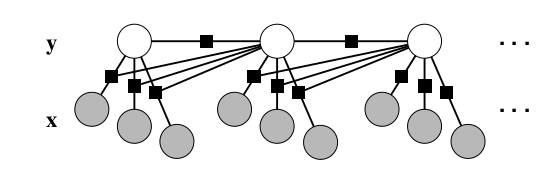
\includegraphics[width=0.7\textwidth]{Bilder/crf-modell-charles-andrew}
\caption{CRF-Modell (die Abbildung ist der Arbeit von Charles Sutton \cite{Charles/Andrew:10} entnommen)}
\label{fig:CRF-Modell}
\end{figure}

\paragraph{}
Die Formel, die die Verteilung $p(y|x)$ beschreibt, lautet 
$$
p(y|x) = \frac{1}{Z(x)}\prod_{t=1}^T\exp \lbrace \sum_{k=1}^K \theta_k f_k(y_t,y_t-1,x_t) \rbrace
$$  

Funktion $f_k$ beschreibt dabei Features, und Vektor $\theta$ - Parameter. Die Funktion $Z(x)$ ist eine Normalisierungsfunktiuon, und wird wie folgt definiert:
$$
Z(x) = \sum_y \prod_{t=1}^T\exp \lbrace \sum_{k=1}^K \theta_k f_k(y_t,y_t-1,x_t) \rbrace
$$
Vektor $x_t$ beinhaltet dabei alle Features, die benötigt werden, um Abhängigkeiten zu berechnen. 

\paragraph{}
Aber wie definiert man Features? Jenny Finkel\cite{Jenny/etal:07} hat folgende Eigenschaften definiert:
\begin{enumerate}
\item Nachbarnwörter: vorheriges Wort, nächstes Wort, alle Wörter innerhalb eines Fensters.
\item Orthographische Eigenschaften.
\item Präfixe und Suffixe.
\item Labelsequenzen.
\end{enumerate}

\subsection{SVM}
\paragraph{}
Support Vector Machines (oder Stützvektormaschine) ist eine Methode zur Klassifizierung von Daten, deren Grundidee\cite{meyer2014support} auf der Abbildung \ref{fig:SVM-INTRO} graphisch dargestellt ist. 

\begin{figure}
\centering
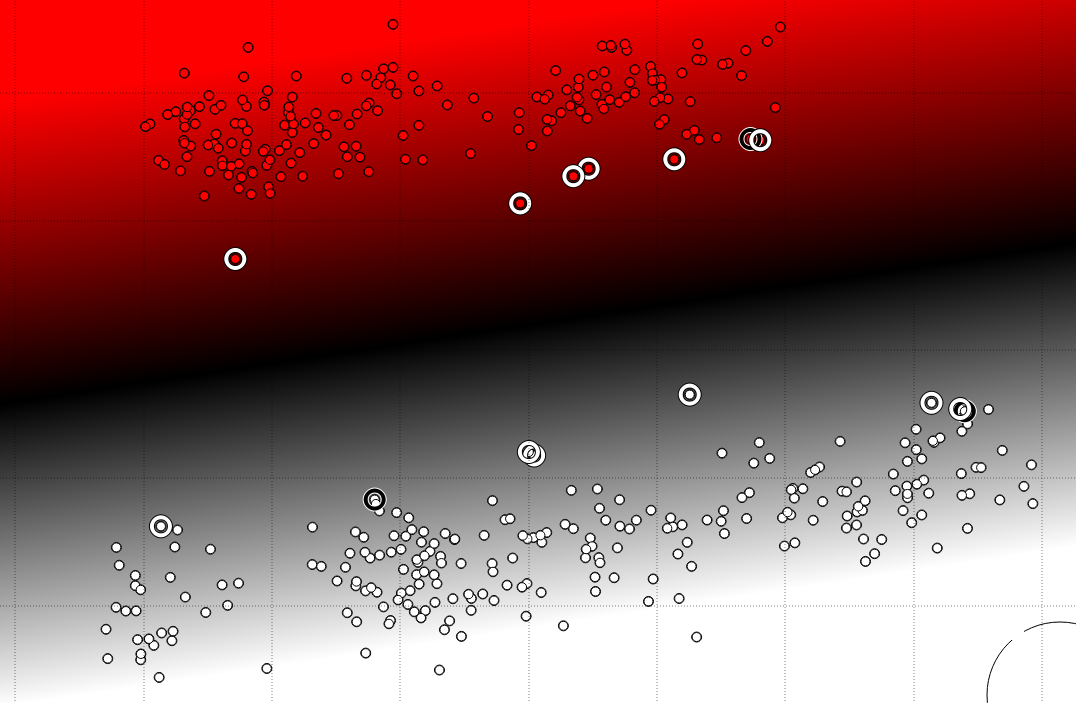
\includegraphics[width=\textwidth,angle=90]{Bilder/svm-intro.png}
\caption{''Die Klassifizierung mithilfe von Stützvektoren''}
\label{fig:SVM-INTRO}
\end{figure}

Der SVM-Klassifikator versucht, für eine Menge von \textbf{linear trennbaren} Punkten in einem Vektorraum eine Hyperebene zu finden, die die Punkte in zwei Klassen aufteilt, und zwar so, dass der Abstand zwischen dieser Trennfläche und den Randpunkten möglichst maximal bleibt.

\paragraph{}
Damit so eine Hyperebene aufgebaut werden könnte, ist es wichtig, dass die Datenpunkte linear trennbar sind. Wenn das SVM-Algorithmus direkt auf nicht linear trennbare Daten angewendet wird, wird die resultierende Trennebene falsch aufgebaut, was auf der Abbildung \ref{fig:SVM-NONLINEAR-ISSUE} zu sehen ist. 

Allerdings sind meiste Daten, mit denen man in der realen Welt arbeiten muss, nicht linear trennbar, und damit kann das SVM-Algorithmus nicht in seiner ursprünglichen Form verwendet werden. Allerdings gibt es eine Möglichkeit, mit einer Erweiterung von SVM-Einsatz auch nicht linear trennbare Daten zu klassifizieren. Dazu muss das ursprüngliche Eigenschaftensraum auf ein Raum höherer Dimension abgebildet werden, und zwar so, dass die Datenpunkte in neuem Raum linear trennbar wären\cite{Hearst:98}.

Das Verfahren, das solche Abbildung ermöglicht, heißt ,,Kernel``, und ist in der Arbeit von Hsu\cite{hsu2003practical} beschrieben. Ein Kern ist eine Funktion 
$K(x_i,x_j) = \phi(x_i)^T \phi(x_j)$, die den Punkt im ursprünglichen Raum $R^{n_1}$ auf ein Punkt im Raum $R^{n_2}$ abbildet, so dass $n_1 < n_2$ ist. In der Praxis sind laut Hsu\cite{hsu2003practical} folgende Kernfunktionen etabliert:
\begin{enumerate}
\item Lineares Kern: $K(x_i,x_j) = x_i^T x_j$
\item Polynominales Kern: $K(x_i,x_j) = (\gamma x_i^T x_j + r)^d, \gamma > 0$
\item Radiale Basisfunktion (RBF): $K(x_i,x_j) = exp(-\gamma \Vert x_i - x_j \Vert^2), \gamma > 0$
\item Sigmoid : $K(x_i,x_j) = tanh(\gamma x_i^T x_j + r)$
\end{enumerate}
Die Variablen $\gamma$, $r$ und $d$ sind benutzerdefinierte Kernelparameter.

\begin{figure}
\centering
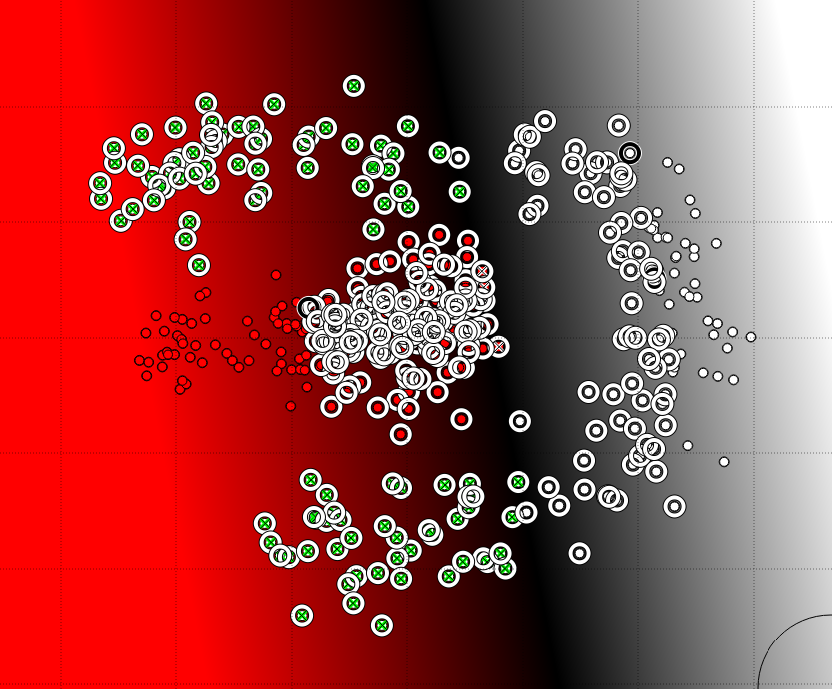
\includegraphics[width=\textwidth,angle=90]{Bilder/svm-nonlinear-issue.png}
\caption{''SVM Algorithmus angewandt auf nicht linear trennbare Daten''}
\label{fig:SVM-NONLINEAR-ISSUE}
\end{figure}

\begin{figure}
\centering
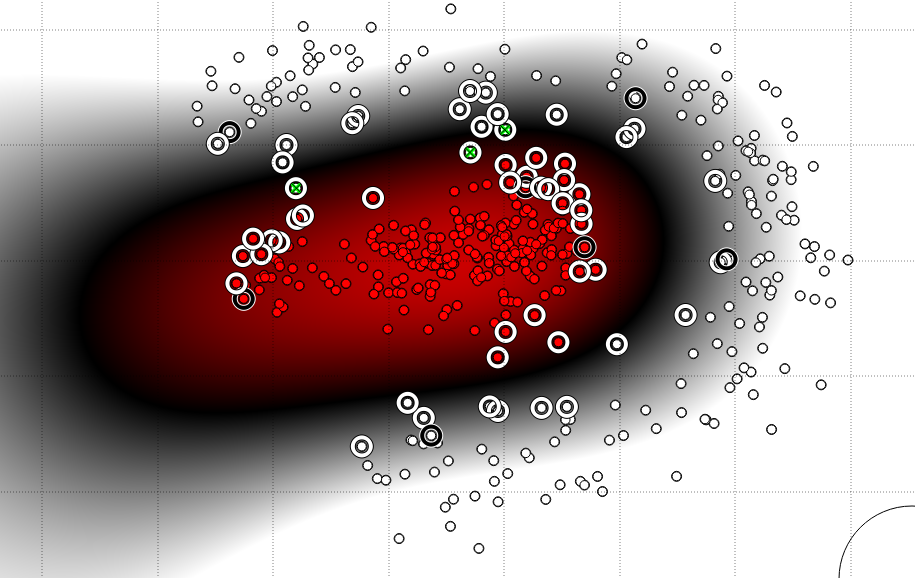
\includegraphics[width=\textwidth,angle=90]{Bilder/svm-nonlinear-rbf.png}
\caption{''SVM-Algorithmus mit einem RBF-Kern angewandt auf nicht linear trennbare Daten''}
\label{fig:SVM-NONLINEAR-ISSUE}
\end{figure}

\paragraph{}
%Und wie kann man SVMs in NEr einsetzen?
Der Einsatz von Stützvektoren für Extraktion von Entitäten ist in der Arbeit von Kazama\cite{kazama2002tuning} beschrieben. Obwohl es in dieser Arbeit um Extraktion von Entitäten aus englischsprachigen medizinischen Texten geht, kann dasselbe Prinzip auch auf deutsche Texte angewendet werden, wenn man das richtige Korpus für Training zur Verfügung stellt. Um SVMs für Extraktion von Entitäten einsetzen zu können, muss noch eine Erweiterung zum ursprünglichen Algorithmus gemacht werden, zusätzlich zum Kerneleinsatz - Stützvektoren können generell zwischen zwei Klassen von Objekten unterscheiden (ein Stützvektoreinsatz kann sagen, ob das Objekt der Klasse $C_a$ oder der Klasse $C_b$ gehört), und bei Entitäten gibt es mehr als zwei Klassen. Um diese Beschränkung umzugehen, wird SVM-Algorithmus auf eine der folgenden Arten und Weisen erweitert:

\begin{itemize}
\item Für jede mögliche Entitätsklasse wird ein SVM aufgebaut, der entscheidet, ob das Token der Klasse $C_a$ oder dem Rest der Klassen gehört.
\item Für jede Paar $(C_a, C_b)$ von möglichen Entitätstypen wird ein SVM erzeugt, der feststellen muss, ob das Wort den Typ $C_a$ oder $C_b$ hat. Die Klasse, die von der Mehrheit von SVMs gewählt wurde, gewinnt.
\end{itemize}

\paragraph{}
Vorteile von SVM-Einsatz anderen Methoden gegenüber:
\begin{itemize}
\item A
\end{itemize}

Nachteile von SVMs anderen Einsätzen gegenüber:
\begin{itemize}
\item B
\end{itemize}

\subsection{Maximum Entropy based NER}
%Was ist ME NER? Wo wird er verwendet? Welche Vor- und Nachteile hat dieser Einsatz im Vergleich zum CRF?
\paragraph{}
Dieses Framework wurde in der Arbeit von Andrew Borthwick\cite{Andrew:99} vorgestellt. In diesem Modell wird auch wie im CRF mit der Wahrscheinlichkeit $p(y|x)$ gearbeitet, allerdings ist ME NER kein graphisches Framework. Die Formell, die die Verteilung für ME-Modell beschreibt, sieht wie folgt aus:
$$
P(y|x) = \frac{1}{Z(x)}\prod_i \alpha_i^{g_i(x,y)}
$$
$g_i$ ist eine binäre Funktion, die eine bestimmte Feature beschreibt, und $\alpha_i$ ist das Parameter, der mit der Eigenschaft assoziiert wird. $Z(x)$ ist eine Normalisierungsfunktion, die wie folgt aussieht:
$$
Z(x) = \sum_y \prod_i \alpha_i^{g_i(x,y)}
$$

\subsection{Features}
Eigenschaften können in zwei Klassen geteilt werden: lokale und globale Features. Hai und Hwee\cite{Hai/Hwee:02} definieren unter anderem folgende Eigenschaften, die auch im OpenNLP-Framework eingesetzt werden:
\begin{enumerate}
\item Globale Eigenschaften:
\begin{enumerate}
\item Personenpräfixe für bestimmtes Wort in anderen Sätzen des Dokumentes: z.B. wenn wir im Text zuerst die Tokens ,,Frau Sony`` treffen, und dann einfach ,,Sony``, dann soll angenommen werden, dass ,,Sony`` eine Entität mit dem Typ ,,Person`` ist.
\item Abkürzungen: wenn in einem Satz mehr Wörter nacheinander groß geschrieben werden, wie z.B. ,,Deutsche Demokratische Republik``, dann wird in dem Text nach entsprechender Abkürzung gesucht: ,,DDR``, und wenn Abkürzung eine Entität ist, können auch alle entsprechende Tokens als eine Entität markiert werden.
\end{enumerate}
\item Lokale Eigenschaften:
\begin{enumerate}
\item Ob das Wort großgeschrieben wird.
\item Ob vorheriges oder nächstes Wort großgeschrieben wird.
\item Ob alle Zeichen im Token großgeschrieben werden.
\item Ob es ein Punkt am Ende des Wortes steht.
\item Ob der Token Zahlen beinhaltet, und falls ja, wie viel.
\item Ob das Wort das Prozent- oder Dollarzeichen beinhaltet.
\item Suffixe und Präfixe (wie ,,Frau`` oder ,,GmbH``).
\end{enumerate}
\end{enumerate}

\section{Wissendatenbanke}
%Was sind Wissendatenbanke? Wieso brauchen wir die in unserer Arbeit? Wie sucht man nach Entitäten in einer Wissendatenbank? Kurze Einleitung in SPARQL+RDF.
\paragraph{}
Um die extrahierte Entitäten mit Ontologien anzureichern, braucht man selbstverständlich eine Datenbank, wo alle Informationen zu den Entitäten gespeichert werden. Solche Datenbanken nennt man ,,Wissendatenbanken``. Solche Datenbanke sind keine herkömmliche relationale Datenbanke, da man die Ontologien mit ihrer hierarchischen Struktur zwar auf ein relationales Modell abbilden lassen kann, aber es gibt bessere Datenstrukturen und Anfragesprachen, die die Arbeit mit Ontologien für die Entwickler einfacher machen.

\paragraph{}
Zur Beschreibung von Ontologien dient das RDF-Format\footnote{\url{http://www.w3.org/2001/sw/wiki/RDF}}. Dieses Format basiert auf XML, und gibt dem Entwickler eine einfache Möglichkeit, Hierarchische Daten zu beschrieben. Die Ontologie im RDF-Format kann z.B. wie folgt aussehen:
\lstset{language=XML}
\lstinputlisting[captionpos=b,label={lst:RDFBEISPIEL},caption={Beispiel einer Ontologie im RDF-Format}]{Listings/examplerdf.xml}

\paragraph{}
Als Anfragesprache für RDF wird SPARQL\footnote{\url{http://www.w3.org/2001/sw/wiki/SPARQL}} eingesetzt. Diese Sprache sieht SQL ähnlich aus, operiert allerdings nicht auf relationalen Daten, sondern auf RDF-Graphen. 

Zum Beispiel, wenn die Fläche der Stadt Duisburg und das Bundesland, wo die Stadt liegt, gebraucht werden, kann die SPARQL-Anfrage wie folgt aussehen:
\lstset{language=SPARQL}
\lstinputlisting[captionpos=b,label={lst:SPARQLBEISPIEL},caption={Beispiel einer SPARQL-Anfrage}]{Listings/sparqlexample.sql}

Die Antwort wird dann im Form eines RDF-Datensatzes geliefert:
\lstset{language=XML}
\lstinputlisting[captionpos=b,label={lst:SPARQLRESULT},caption={Beispiel der Antwort auf eine SPARQL-Anfrage}]{Listings/sparqlresult.xml}